\documentclass[a4paper, 12pt, uplatex]{jsarticle}


\usepackage{amsthm}
\usepackage{amsmath}
\usepackage{amssymb}
\usepackage{amsfonts}
\usepackage{thmtools}
\usepackage{bm}
\usepackage[margin=1cm, includefoot]{geometry}
\usepackage[dvipdfmx]{graphicx}
\usepackage[dvipdfmx]{xcolor}

\usepackage[hyphens]{url}
\usepackage{url}

\usepackage{float}
\usepackage[dvipdfmx]{hyperref, graphicx}
\usepackage{pxjahyper}
\hypersetup{
	colorlinks=false, % リンクに色をつけない設定
	bookmarks=true, % 以下ブックマークに関する設定
	bookmarksnumbered=true,
	pdfborder={0 0 0},
	bookmarkstype=toc,
}
\newcommand{\linedhref}[2]{\underline{\href{#1}{\emph{#2}}}}

\declaretheoremstyle[
  spaceabove=6pt, spacebelow=6pt,
  headfont=\bfseries\sffamily,
  notefont=\bfseries\sffamily,
  notebraces={(}{)},
  postheadspace=1em,
  numbered=no,
  qed=\(\square\)
]{myproof}
\declaretheorem[title=証明, style=myproof]{myproof}
\renewenvironment{proof}{\begin{myproof}}{\end{myproof}}

\usepackage{minted}
\renewcommand{\listingscaption}{ソースコード}
\usemintedstyle{monokai}
\definecolor{monokaibg}{HTML}{282828}
\setminted{bgcolor=monokaibg}
\definecolor{Text}{HTML}{F8F8F2}
\AtBeginEnvironment{minted}{\color{Text}}


\author{0000000000-0 \\ レポート 太郎}
\title{\LaTeX 実践1\\第1回\\レポート課題 \LaTeX のサンプル}
\date{}

\begin{document}

\maketitle

\begin{abstract}
  このレポートは,\LaTeX でレポートを書くサンプルである.
\end{abstract}

\section{背景}
レポートを \LaTeX で書こう.

\section{サンプル}

\subsection{段落}

行を開けると,段落になる.

山路を登りながら.

\subsection{数式}
Albert Einstein の特殊相対論によれば,エネルギー \(E\) と質量 \(m\) は
\[
  E = mc^{2}
\]
で関係づけられる.

\subsection{画像}


画像のサンプルを,図 \ref{fig:image} に示す.

\begin{figure}[ht]
  \begin{center}
    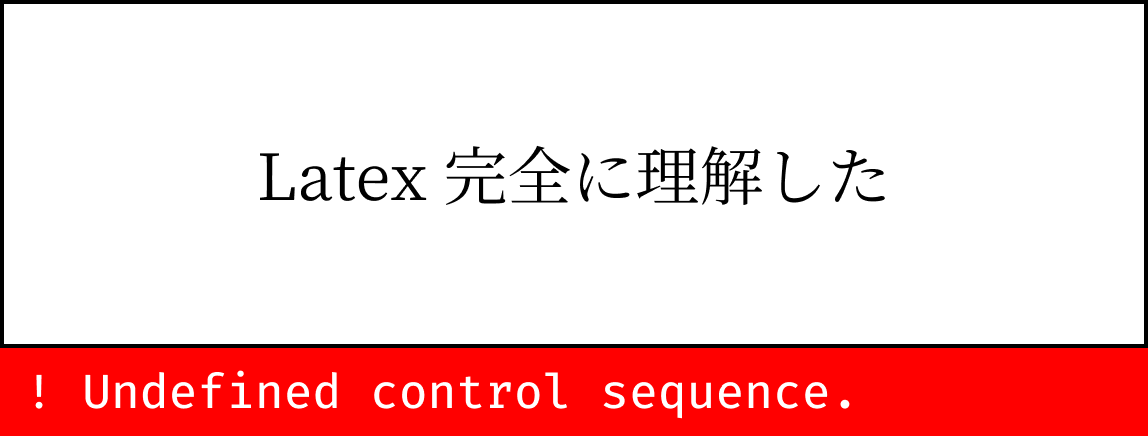
\includegraphics[width=0.4\linewidth]{image.png}
  \end{center}
  \caption{画像のサンプル}
  \label{fig:image}
\end{figure}

\subsection{ソースコード}

JavaScript で \texttt{console.log} 関数 \cite{consolel20:online} を呼び出す,
ソースコードのサンプルを,ソースコード \ref{lst:js} に示す.


\begin{listing}[ht]
  \begin{minted}{js}
console.log("こんにちは!");
  \end{minted}
  \caption{ソースコードのサンプル}
  \label{lst:js}
\end{listing}

\subsection{TextLint}

次の段落は,TextLint によってエラーとなる.

こんにちわ.TextLint のサンプルです。


\bibliography{bib}
\bibliographystyle{junsrt}

\end{document}
